\chapter{Algorithms and Implementation}

\section{Interface Implementation}\label{interface-implementation}

One of the core components of Foldlings is the interface. To create
features, we capture touch input, display a preview of the fold feature
as the user creates it, and add created features to the fold pattern.
This system is outlined in Figure \ref{mvc}.

\begin{figure}[htbp]
\centering
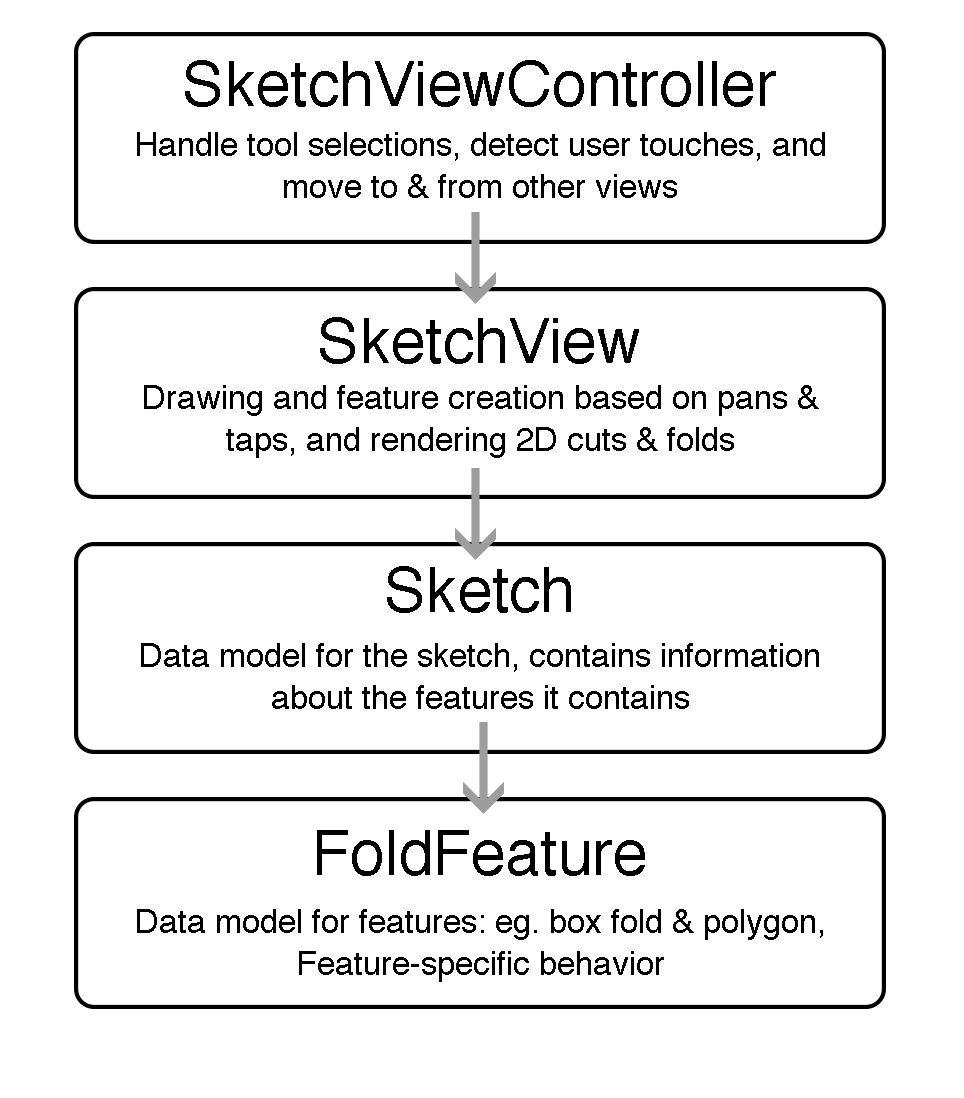
\includegraphics{figures/40_Tech_Interface_Implementation/sketchview-descendents-thesis-figure.png}
\caption{Relationship between interface classes: a SketchViewController
manages a SketchView that contains a Sketch that contains FoldFeatures.
\label{mvc}}
\end{figure}

Although this structure borrows heavily from the Model-View-Controller
design pattern, we do not follow the pattern strictly. The MVC paradigm
often becomes muddy, with much information shared between the separate
modules (\citet{veit2003model}). In our case, we separate modules not
purely based on MVC encapsulation but based on functionality. For
example, rather that strictly separating all touch handling into the
view controller or all drawing into the view, these responsibilities are
shared between the classes as needed to perform their roles. See section
\ref{touch-handling} for more information.

\subsection{Tool Selection}\label{tool-selection}

Tool state is maintained by the SketchViewController.

\subsection{Touch Handling}\label{touch-handling}

In order to create features, we first need to capture touch input.
Foldings handle two types of touches:\\catmull rom curves

\textbf{\textgreater{}\textgreater{}TODO: CITE APPLE DOCS}

\subsection{Fold Feature Preview}\label{fold-feature-preview}

While, the SketchView must display a

description of drawing, touch handling, etc.

Drawing in progress Drawing features already in the sketch

\subsection{Feature Creation}\label{feature-creation}

showing feature state Shading planes

Once the suer completes a feature, we add it to the sketch\footnote{Assuming
  the feature is valid. \textbf{\textgreater{}\textgreater{}TODO: cite
  validity}}. The feature-specific implementations of the FoldFeature
superclass are described in Chapter \ref{tool-implementation} on page
\pageref{tool-implementation}. The Sketch class contains methods for
adding and removing features from the sketch. It also contains
lower-level functions for adding, removing, and replacing edges. These
methods are typically called by feature-specific methods that modify the
sketch.
